\documentclass[12pt]{article}

\usepackage{listings}
\lstset{
  language=Haskell
}

\usepackage{graphicx}
\graphicspath{ {../resources/tic-hack-toe/} }

\usepackage[margin=1in]{geometry}

\usepackage[colorlinks]{hyperref}
\hypersetup{
  urlcolor = {cyan}
}

\title{Hack the North Part 1 - Tic Hack Toe}
\author{Rushi Shah}
\date{19 September 2015}

\begin{document}

  \maketitle

  \begin{center}
  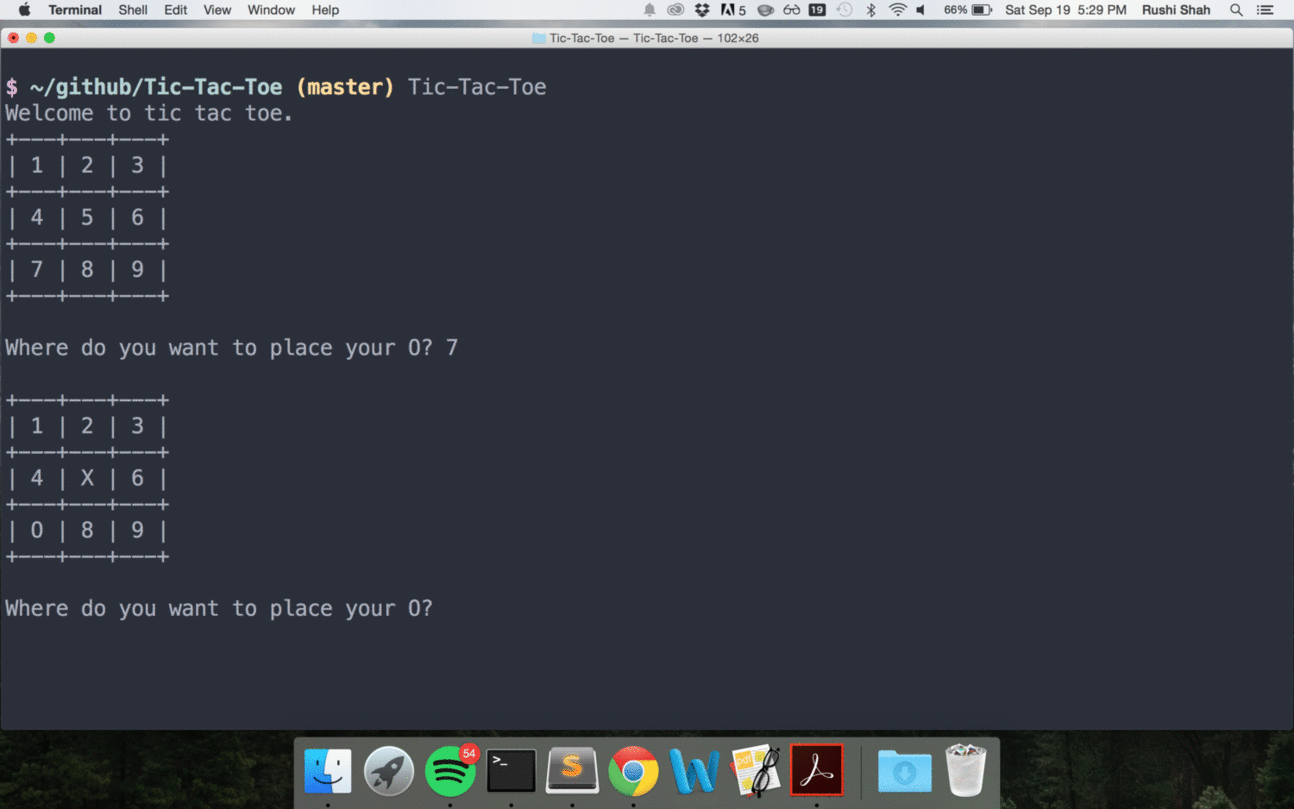
\includegraphics[width=6in]{screen_shot}
  \end{center}

  Hack the North 2014 was where it all began. Sure, it was technically my
  second hackathon, but it was my first collegiate hackathon (I was a
  junior in high school) and it was my first international hackathon. Well
  Canada has done it again, because Hack the North 2015 has been great so
  far (it is about 1AM on Sunday morning).

  My team and I were vacillating about ideas for most of Friday night and
  Saturday morning so in my spare time I continued learning the dark arts
  of Haskell. I decided to make a project rather than just chugging
  through CIS194 (partially because I was stumped). Since I had so much
  fun making a \href{https://github.com/2016rshah/sudoku-solver}{sudoku
  solver} in Haskell, I decided to make a Tic-Tac-Toe game. Just a simple
  terminal gui and a decent computer AI for anybody who wants to take a
  quick break while coding, you know?

  Well boy was it a learning experience. For example, this was the first
  project that I created without that much outside structure in Haskell.
  Even with the Sudoku solver, I followed an assignment sheet for a sort
  of roadmap. But I was flying solo on this one, which was liberating!

  The project itself was split up into two separate parts. First of all,
  the game mechanics and the AI of tic-tac-toe, and second of all the
  user-input/interface. Typically in an imperative language, the I/O is
  the easy part, and the AI is the hard part. But that was not the case
  with this project.

  \section{The Game Mechanics and the
  AI}\label{the-game-mechanics-and-the-ai}

  I just followed this
  \href{http://programmers.stackexchange.com/questions/213559/algorithm-to-create-an-tictactoe-game-ai}{general
  outline} on the decision tree for the program. It was surprisingly easy,
  and a ton of fun to code. Most of the AI code is in the
  \href{https://github.com/2016rshah/Tic-Hack-Toe/blob/master/src/TicTacToe.hs}{TicTacToe
  module}.

  \section{The Input/Output}\label{the-inputoutput}

  In python, this would be a synch. Just
  \texttt{location\ =\ input("Where\ do\ you\ want\ to\ move?")} and wrap
  the game loop in a while loop until someone wins or the game draws.
  Haskell is very different, but as I learned, not necessarily more
  difficult. Loops and mutable variables are a no no so I was stumped for
  a short amount of time.

  I read a lot about fancy solutions like
  \href{http://projects.haskell.org/operational/examples/TicTacToe.hs.html}{Monads},
  but I thought that was overkill and I thought that there must be a
  better solution. After testing out my functions with some
  \href{https://github.com/2016rshah/Tic-Hack-Toe/commit/201ef6f4ab5bdcd74675f582dcabe47468d49522}{sketchy
  code}, I decided it was time to
  \href{http://stackoverflow.com/questions/32670948/take-input-from-user-until-tic-tac-toe-game-ends}{ask
  Stack Overflow}.

  \href{http://stackoverflow.com/a/32671373/3861396}{The response} I got
  blew me away. Not only was it very in-depth and well explained, the idea
  was so elegant: mutual recursion between the player's turn and the
  computers turn that simply stops recurring when the game ends! Coming
  from an OOP background, that solution would never have been immediately
  obvious to me, but understanding the solution from both points of view
  makes me feel almost enlightened. That's the beauty of functional code.
  It doesn't necessarily have to be better or worse, just different.

  Most of the IO code is in the
  \href{https://github.com/2016rshah/Tic-Hack-Toe/blob/master/src/Main.hs}{Main
  module}.

  \section{Hackage Package}\label{hackage-package}

  The last thing I did was push
  \href{https://hackage.haskell.org/package/Tic-Tac-Toe-0.1.0.2}{the
  project on to Hackage}, which is Haskell's package manager. This was my
  first time publishing my work on any sort of package manager at all, so
  this was just another adventure. It was surprisingly easy because mostly
  everything had already been set up using
  \href{https://github.com/khanage/heineken}{heineken} (which is so
  awesome), it just involved changing a few config files. One of the most
  frustrating parts was when everything was working locally but breaking
  when I installed from hackage and I couldn't figure out why. Turns out I
  needed to declare the TicTacToe module in the cabal file, so adding
  \texttt{other-modules:\ TicTacToe} fixed everything. I also followed
  this
  \href{http://begriffs.com/posts/2014-10-25-creating-package-hackage.html}{guide
  on publishing to hackage} to make sure everything would go smoothly, in
  case you are interested in publishing some of your code. What's the
  moral of the story? The moral of the story is that you can install
  Tic-Hack-Toe!

  Just run

  \begin{lstlisting}
  > cabal update 
  > cabal install Tic-Tac-Toe 
  > Tic-Tac-Toe
  \end{lstlisting}

\end{document}